% Chapter 2

% % % % Some Macros 

\newcommand{\laplacian}[1][G]{\ensuremath{L_{#1}^{+}}}
\newcommand{\reffformula}[1][\laplacian]{\ensuremath{ (\chi_u - \chi_v)^T \  #1 \ (\chi_u - \chi_v) }}
\newcommand{\reff}[1][e]{\ensuremath{R_#1^{\text{eff}}}}
\newcommand{\proj}{\ensuremath{I - \frac{\textbf{1} \textbf{1}^T}{n}}}
\newcommand{\sqlaplacian}[1][G]{\ensuremath{\sqrt{L_{#1}^{+}}}}
\newcommand{\Mset}[2]{\ensuremath{\mathbb{M}_{#1 \times #2}}}

% from https://tex.stackexchange.com/questions/107186/how-to-write-norm-which-adjusts-its-size
\newcommand\norm[1]{\left\lVert#1\right\rVert}
%  


%  from https://tex.stackexchange.com/questions/39390/writing-a-limit-so-that-the-subscript-goes-directly-underneath

\newcommand{\Lim}[1]{\raisebox{0.5ex}{\scalebox{0.8}{$\displaystyle \lim_{#1}\;$}}}

\chapter{Matrix Approach} % Main chapter title

\label{Chapter4} % For referencing the chapter elsewhere, use \ref{Chapter2} 

%----------------------------------------------------------------------------------------
% \section{Colbourn, Day, Nel}

\section{Harvey, Xu}

\cite{harvey2016generating} proposed a $\mathcal{O}(N^\omega)$ (where $\omega$ is the exponent of fast matrix multiplication) algorithm for sampling a uniform spanning tree which is much simpler compared to the one proposed earlier by CMN which also has the same running time. The initial starting point for the algorithm is using the relationship between effective resistance and the probability that an edge belongs to a spanning tree. And also the fact that sampling an edge corresponds to contracting it and discarding the edge corresponds to deleting it. The following naive chain rule algorithm works on the same principle. 

% \subsection{Techniques used}



\subsubsection{Naive chain rule algorithm}




\begin{algorithm}[H]
 \KwIn{$G = (V,E) \  \text{and} \  L_G^+$}
 \KwOut{Set of edges corresponding to a random spanning tree}
 
 \For{$e = (u,v) \in E$ }{
    $R_e^{\text{eff}} = (\chi_u - \chi_v)^T \ L_G^+ \ (\chi_u - \chi_v)$\;
  \eIf{$(X \sim \text{Bernoulli}(R_e^{\text{eff}})) = 1$} {
   Add edge $e$ to the spanning tree\;
   $G = G / e$\;
   }{
   $G = G \setminus e$ \;
  }
  Update $ L_G^+ $ \;
 }
 \caption{Sampling uniform spanning tree using chain rule}
\end{algorithm}

Computing $\laplacian$ takes $\mathcal{O}(N^3)$ hence the overall running time is $\mathcal{O}(MN^3)$

\subsection{Summary of the paper}

On a high level the main ideas used in the paper are 

\begin{enumerate}
 \item Use a divide and conquer algorithm to break the graph into smaller parts and sample on each parts seperately and update the pseudoinverse of the laplacian lazily only on the subgraph when needed
 \item The important insight here is that the sampling probability of an edge depends only on 4 entries of the pseudoinverse of the laplacian. Hence we don't need to update all the entries of the matrix when the graph is modified
 \item A well known method to compute inverse of a matrix with updates is to use the Sherman-Morrison-Woodbury formula. But in this case the formula has to be modified to work for the case where only a submatrix is modified.
 \item Since while contracting an edge the number of vertices decreases it would get cumbersome to modify the dimension of the matrix evertime. So they overcome this issue by considering the formula on the limit case. When the graph is considered as a electric network then increasing the weight of an edge corresponds to shorting that link, hence in the limit case we get the same result as contracting the edge
\item Also one of the main improvements over the previous algorithms (\cite{COLBOURN1996268}) is that the intricacies of LU decomposition is avoided since the current algorithm uses only matrix inversion as black box. 
\end{enumerate}

\subsection{Harvey, Xu Algorithm}

(TODO) Insert algorithm here and explain how it works
\begin{center}
    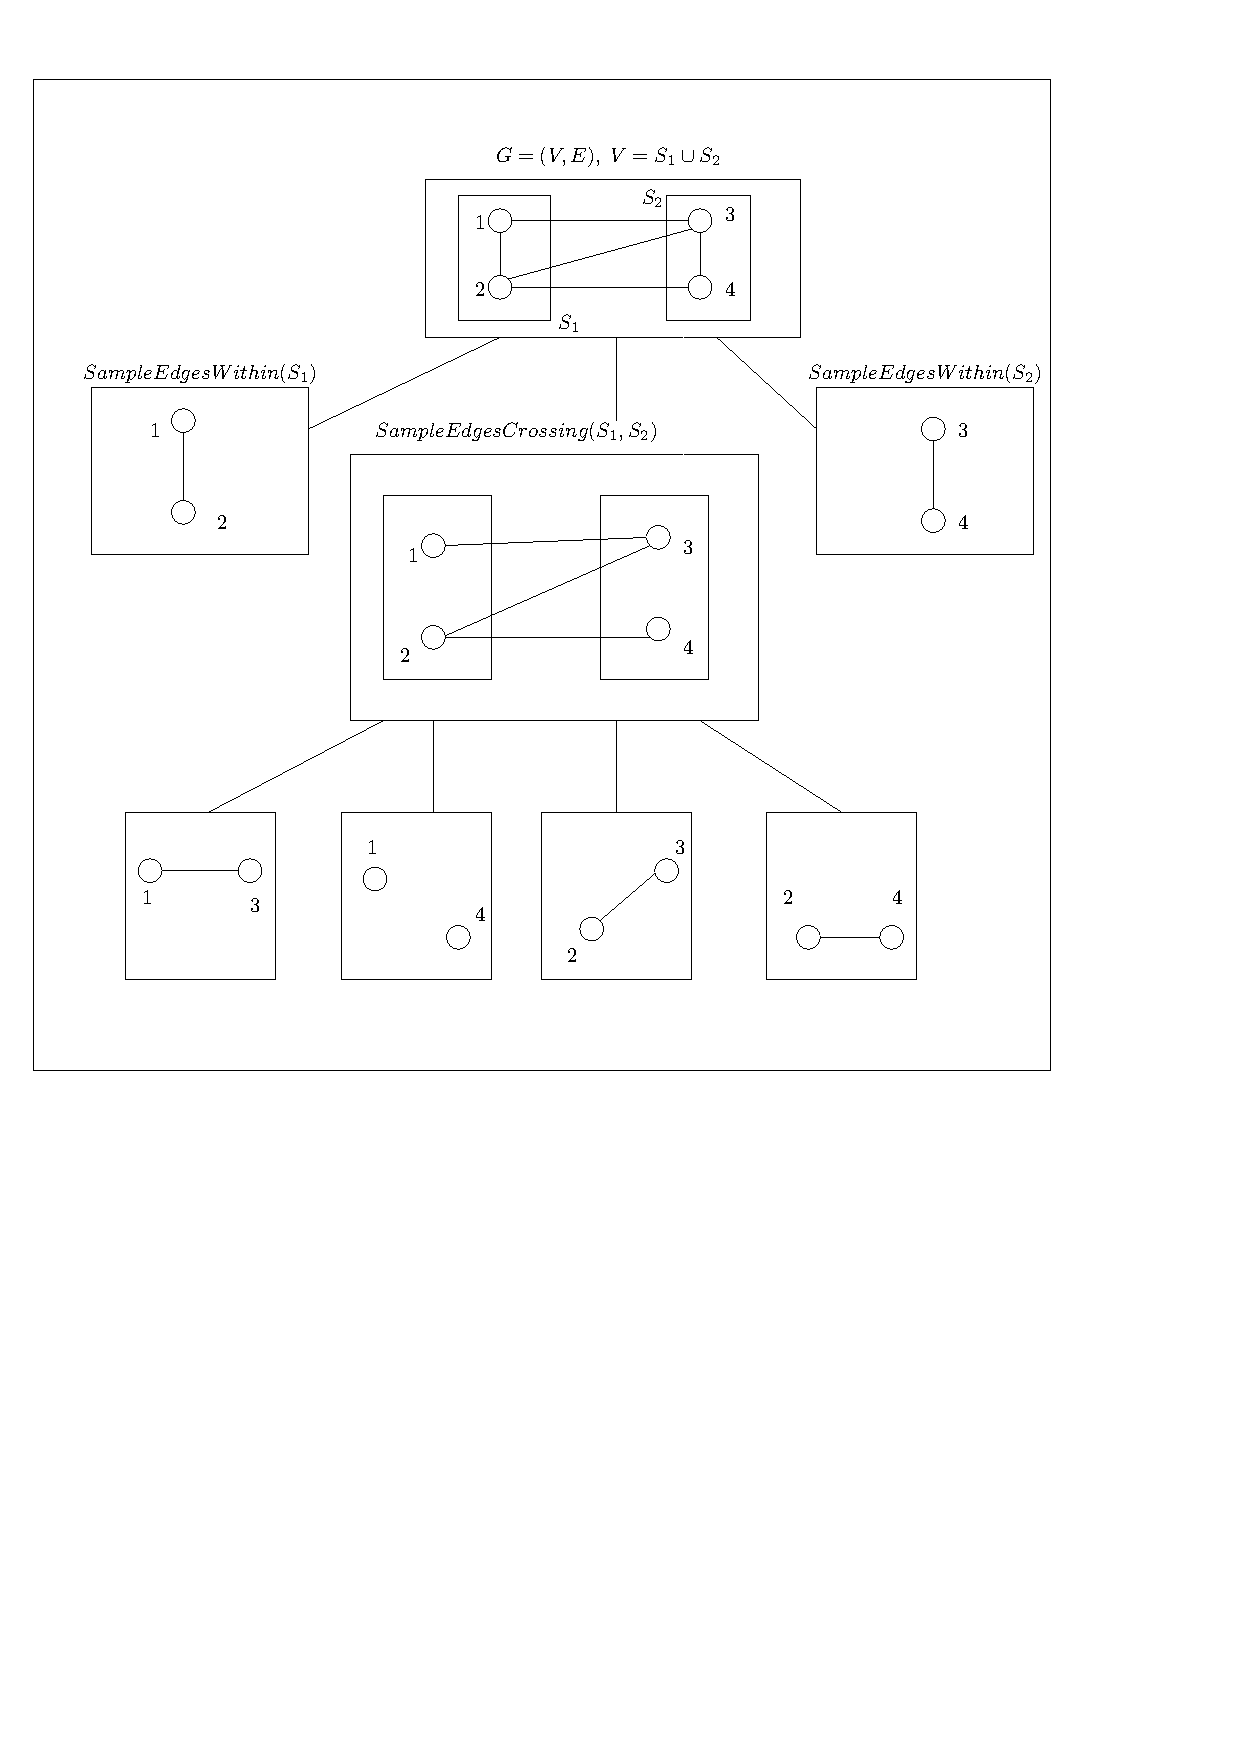
\includegraphics[scale=0.85]{Figures/alg-tree}
\end{center}



\subsection{Structure of the paper}

\begin{center}
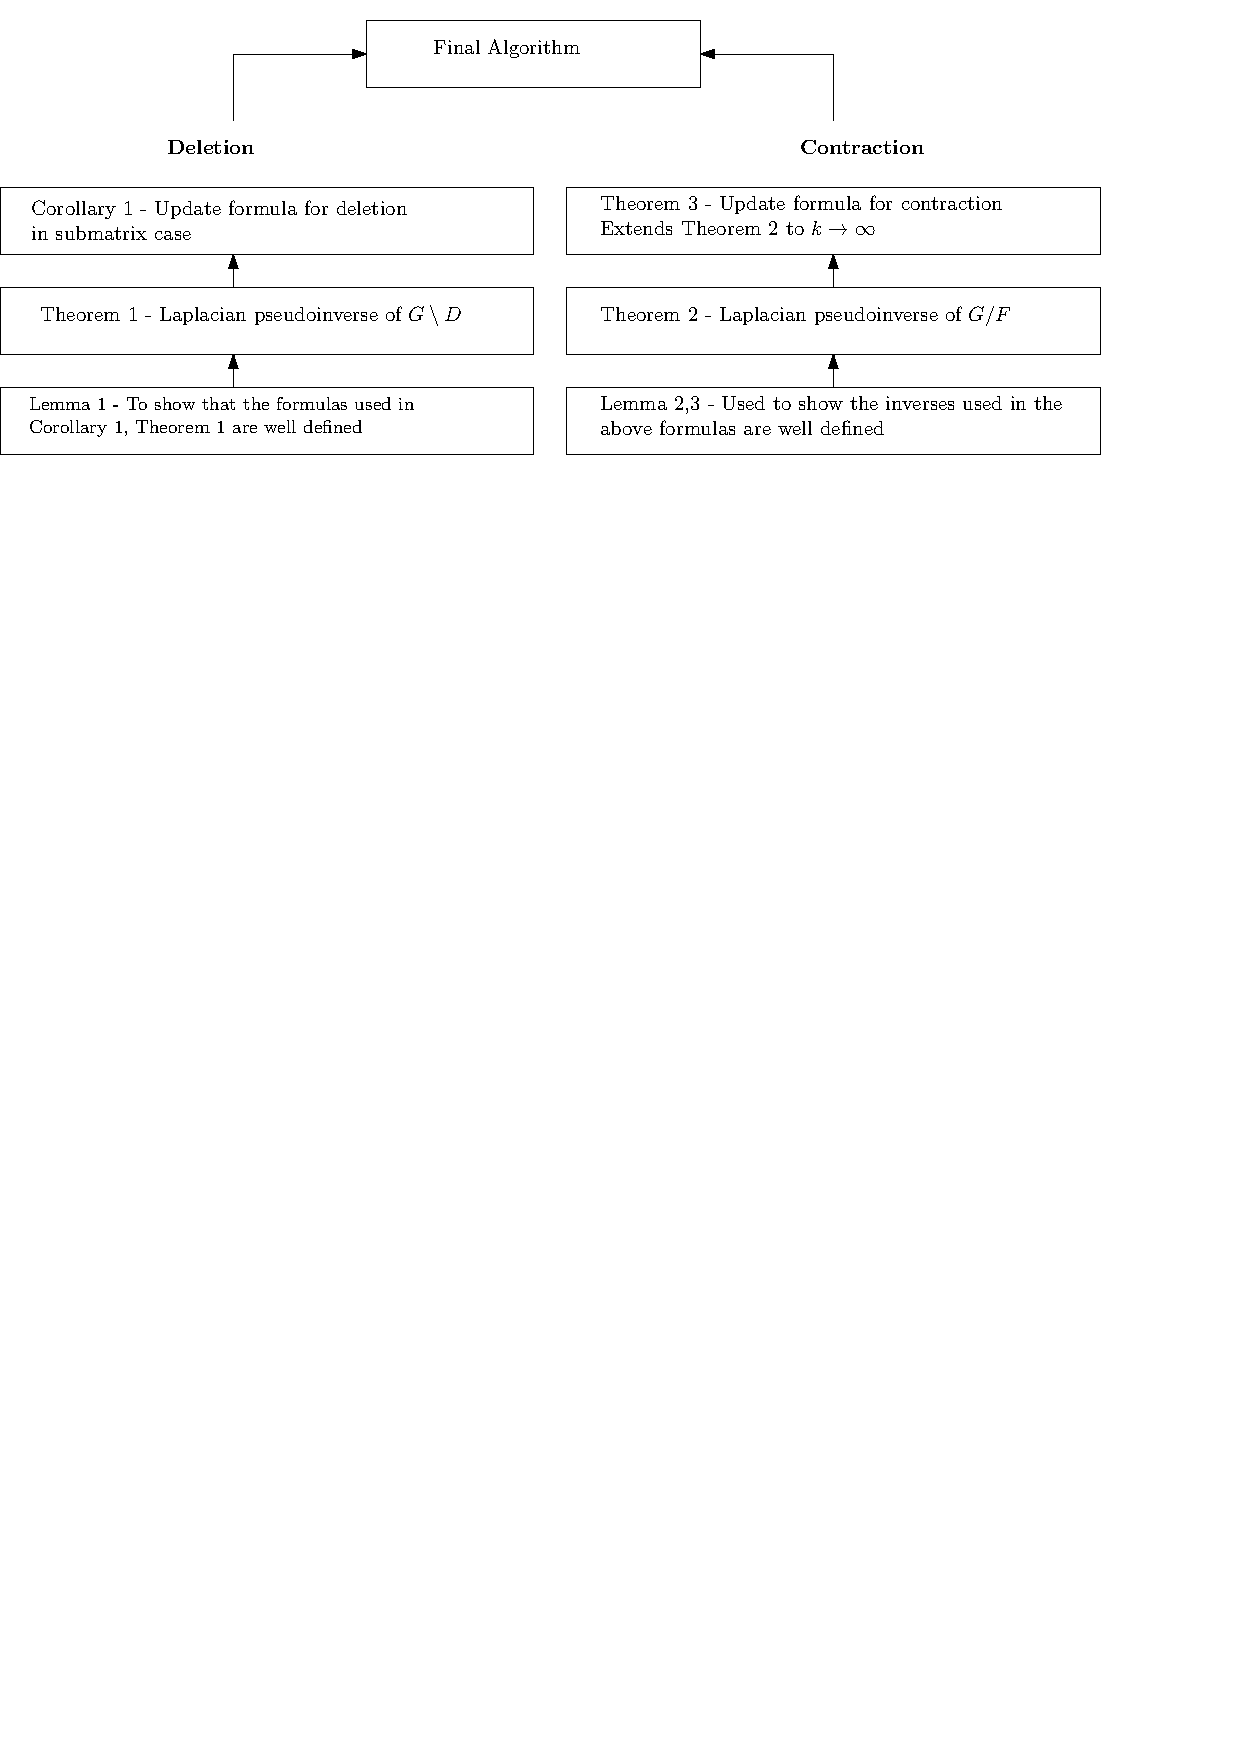
\includegraphics[scale=0.7]{deps} 
\end{center}


\subsection{Facts used}

\begin{HXf}[Woodbury matrix identity]
 Let $ M \in \mathbb{M}_{n \times n} , U \in \mathbb{M}_{n \times k}, V \in \mathbb{M}_{n \times k}$. Suppose $M$ is non-singular then $M + UV^T$ is non-singular $\iff \ I + V^T M^{-1} U$ is non-singular. If $M + UV^T$ is non-singular, then 
 $$ (M + UV^T)^{-1} = M^{-1} - \left( M^{-1} \cdot U \cdot (I + V^TM^{-1}U)^{-1} \cdot V^T \cdot M^{-1}\right) $$
\end{HXf}

% \begin{proof}
%  TODO
% \end{proof}

\begin{HXf}
 For any $L \in \mathbb{M}_{n \times n}$ with $\text{ker}(L) = \text{span}(\textbf{1})$, we have $LL^+ = I - \frac{\textbf{1} \cdot \textbf{1}^T}{n}$ and $P := I - \frac{\textbf{1} \cdot \textbf{1}^T}{n}$ is called the \textbf{projection matrix}. 
\end{HXf}

The folowing set of facts are about the properties of matrix operations (addition, multiplication, etc.) on sub-matrices. The first 4 are easy to see, so I haven't derived them. For the last one I have written a derivation using Shur's complement from Wikipedia

\begin{HXf}[Sub-matrices]
For all the results below, $S$ denotes a index set and $S^c$ denotes it's complement.
 \begin{enumerate}
  \item For any $A,B \in \Mset{n}{n}, (A + B)_{S,S} = A_{S,S} + B_{S,S}$
  \item If $C = D \cdot E \cdot F$ then $C_{S,S} = D_{S,*} \cdot E \cdot F_{*,S}$
  \item For $A \in \Mset{m}{n}, B \in \Mset{n}{l}$ , If $A_{S^c, S^c} = 0$ or $B_{S^c, S^c} = 0$ then \\ $(AB)_{S,S} = A_{S,S} \cdot B_{S,S}$
  \item For any matrix $C$ where $C = D \cdot E \cdot F$ . If $D_{*, S^c} = 0$ and $F_{S^c, *} = 0$, then $C = D_{*, S} \cdot E_{S,S} \cdot F_{S,*}$
  \item $D = 
\begin{bmatrix}
M & 0 \\
0 & 0 \\
\end{bmatrix},
$ 
and $
E = 
\begin{bmatrix}
A & B \\
X & Y \\
\end{bmatrix}
$
where $M, A \in \Mset{n}{n}$ and If $(MA - I)$ is invertible Then,
$$ (DE - I)^{-1} = \begin{bmatrix}
(MA - I)^{-1} & (MA - I)^{-1} \cdot M \cdot B \\
0 & -I \\
\end{bmatrix}
$$
\begin{proof}
 $(DE - I)^{-1}$ can be computed using Shur's Complement(\cite{wiki:shur}) . 
 
 Suppse $N =  
\begin{bmatrix}
P & Q \\
R & S \\
\end{bmatrix}
$ and Shur's complement of block $S$ and $P$ is  $$N / S := P - QS^{-1}R \qquad N / P := S - RP^{-1}Q$$
Then $$N^{-1} = 
\begin{bmatrix}
P^{-1} + (P^{-1} Q (N/P)^{-1} R  P^{-1}) & -(P^{-1}Q(N/P)^{-1}) \\[0.3cm]
-((N/P)^{-1}RP^{-1}) & (N/P)^{-1} \\
\end{bmatrix}
$$
In our case $N = 
\begin{bmatrix}
MA - I & MB \\
0 & -I \\
\end{bmatrix}
$ and $(N/P) = -I$. From this it follows that $$N^{-1} = (DE-I)^{-1} = \begin{bmatrix}
(MA - I)^{-1} & (MA - I)^{-1} \cdot M \cdot B \\
0 & -I \\
\end{bmatrix}
$$
\end{proof}

 \end{enumerate}

\end{HXf}

\begin{HXf}
 Let $A, B \in \Mset{n}{n}$ with $B$ being symmetric PSD. Suppose $x$ is an eigenvector of $AB$ corresponding to eigenvalue $\lambda$. Then $\sqrt{B} x$ is an eigenvector of $\sqrt{B}A\sqrt{B}$ corresponding to eigenvalue $\lambda$ 
\end{HXf}

\begin{HXf}[Laplacian and graph connectivity (Fiedler value)]
 Let $G$ be a graph with $n$ vertices. Suppose $(\lambda_1, \lambda_2 \cdots \lambda_n)$ be the eigenvalues corresponding to the eigenvectors $(v_1, v_2 \cdots v_n) $ of the Laplacian of $G$ denoted as $L_G$. $L_G$ is symmetric PSD with $\lambda_1 = 0$ and $v_1 = \textbf{1}$. The following properties relate the eigenvalues of $L_G$ with the connectivity of $G$ :
 
\begin{enumerate}
 \item $\lambda_2 > 0 \iff G$ is connected
 \item $G$ is disconnected $\iff \exists z$ with $z^T \textbf{1} = 0$ and $z^T L_G z = 0$
\end{enumerate}

The above is true for $\laplacian$ also 
 
\end{HXf}


 \begin{HXd}[$\chi_u$]
 $\chi_u$ is a vector of size $|V|$

 \[
    \chi_u(i) = 
\begin{cases}
    1,& \text{if } i = u\\
    0,              & \text{otherwise}
\end{cases}
\]
 \end{HXd}

 \begin{HXd}[Uniform random spanning tree]
  Let $\hat{T}$ be the random variable denoting a uniformly random spanning tree, then $\mathbb{P}(\hat{T} = T) = \frac{1}{|\mathcal{T}|}$, where $\mathcal{T}$ is the set of all spanning trees of $G$. 
 \end{HXd}


\begin{HXf}
 Given a graph $G = (V,E)$ with laplacian $L_G$, the effective resistance of an edge $e = \{u, v\} \in E$ is 
 $$ \reff = \reffformula $$
 
 Then for any $e \in E$ we have $$\mathbb{P}(e \in \hat{T}) = \reff$$
 
\end{HXf}








\subsection{Technical details of the results}

\subsubsection{Deletion}
The first step in obtaining a updation formula for deletion is to make sure $(I - L_D \laplacian)$ is invertible. As the inverse of this term would be used in the expansion of $(L_G - L_D)^+$


For the first direction of Lemma 1, the main result used is \textbf{Fact 5} ($G$ is disconnected $\iff \exists z$ with $z^T \textbf{1} = 0$ and $z^T \laplacian z = 0$). So if we can show this for a suitable $z$ we are done. Now using the hypothesis that $(I - L_D \laplacian)$ is singular and \textbf{Fact 4} they derive the following $ y^T \cdot \sqlaplacian \cdot L_{G \setminus D} \cdot \sqlaplacian \cdot y = 0$. As we an see the remaining part is to show $(z = \sqlaplacian y) \perp \textbf{1}$


\begin{HXl}[Formulas in \textbf{Theorem 1} are well defined]
  Let $G=(V,E)$ be a connected graph and $D \subseteq E$ then  
  
  $\left( I - L_D \laplacian \right)$ is invertible $\iff G \setminus D$ is connected 
  
\end{HXl}

\begin{proof}



 First let's show that If $(I - L_D\laplacian)$ is singular then $G \setminus D$ is disconnected 
 
 \begin{itemize}
  \item Since $(I - L_D\laplacian)$ is singular $\exists x \neq 0 \text{ s.t. }$ $(I - L_D\laplacian)x = 0$
  \begin{alignat}{1}
   & \implies L_D \laplacian \ x = x \\
   & \implies 1 \in eigenvalues(L_D\laplacian) \\
   & \implies 1 \in eigenvalues((L_G - L_{G \setminus D}) \laplacian) 
%    & \therefore
  \end{alignat}
  
  \item Let $x \perp \textbf{1}$ be an eigenvector of $(L_G - L_{G \setminus D}) \laplacian$ with eigenvalue 1.
  \item By \textbf{Fact 4}, $y = \frac{\sqrt{\laplacian} x}{\norm{\sqrt{\laplacian}x}}$ is an eigenvector of $\sqrt{\laplacian} (L_G - L_{G \setminus D}) \sqrt{\laplacian}$

\begin{alignat}{1}
   & = y^T \cdot \sqrt{\laplacian} (L_G - L_{G \setminus D}) \sqrt{\laplacian} \cdot y = 1 \\
   & = y^T \sqrt{\laplacian} L_G \sqrt{\laplacian} y = (HOW) y^T \laplacian L_G y = y^T P y  \\
   & = y^T  \left( I - \frac{\textbf{1}^T \textbf{1}}{n} \right) y = y^T y - \left( \frac{y^T \textbf{1}^T \textbf{1} y}{n} \right) = (HOW) y^T y = 1 
\end{alignat}

    \item $\therefore  y^T \sqrt{\laplacian} L_{G \setminus D} \sqrt{\laplacian} y = 0$ now if we consider $z = \sqrt{\laplacian} y$ and show that $z^T \textbf{1} = 0$ then we can use $\textbf{Fact 5}$ to complete the proof
    
    \begin{alignat}{1}
     &  y^T \sqrt{\laplacian} \textbf{1} = x^T \sqrt{\laplacian} \sqrt{\laplacian} \textbf{1} = 0 \text{(HOW is 1 in kernel of } \laplacian \\ 
     &  G \setminus D \text{ is disconnected}
    \end{alignat}

  
 \end{itemize} 

Now to prove the converse, If $G \setminus D$ is disconnected then $I - L_D \laplacian$ is singular

\begin{itemize}
 \item If $G \setminus D$ is disconnected then $\exists y \perp \textbf{1}, ||y|| = 1$ we have
    
%     \begin{alignat}{1}
    \begin{enumerate}
     \item $ y^T \cdot \sqlaplacian \cdot L_{G \setminus D} \cdot \sqlaplacian \cdot y = 0 (HOW) $
     \item $ y^T \cdot \sqlaplacian \cdot L_G \cdot \sqlaplacian \cdot y = y^T y = 1 $
    \end{enumerate}
    
\item From (1) and (2) we get $y^T \sqlaplacian (L_G - L_{G \setminus D}) \sqlaplacian y= 1$
\begin{alignat}{1}
 & \implies y^T \cdot \sqlaplacian \cdot L_D \cdot \sqlaplacian \cdot y = 1 \\
 & \implies 1 \in \text{eigenvalues}(L_D\laplacian) (HOW)\\
 & \implies (I - L_D\laplacian) \text{ is singular}
\end{alignat}

\end{itemize}




\end{proof}



In \textbf{Theorem 1} they just show that the formula for the updated pseudoinverse is indeed true. This is shown using the following identity $L L^+ = P$
\begin{HXt}[Update identity for Deletion] 
 Let $G=(V,E)$ be a connected graph and $D \subseteq E$. If $G \setminus D$ is connected then 
$$ (L_G - L_D)^+ = \laplacian - \left( \laplacian \cdot (L_D\laplacian-I)^{-1} \cdot L_D \cdot \laplacian\right)$$
\end{HXt}

\begin{proof}
 If R.H.S is indeed true then it should satisfy the property of $LL^+ = P$
 $$ (L_G - L_D) \cdot (L_G - L_D)^+ $$
 $$ (L_G - L_D) \cdot \left(\laplacian - \left( \laplacian \cdot (L_D\laplacian-I)^{-1} \cdot L_D \cdot \laplacian\right) \right)$$
 $$\left[P - L_D\laplacian \right] - \left[(L_G\laplacian - L_D\laplacian) \cdot (L_D\laplacian-I)^{-1} \cdot L_D \cdot \laplacian\right]$$
 $$\left[P - L_D\laplacian \right] + \left[\left( (L_D\laplacian - I) + \frac{\textbf{1}\textbf{1}^T}{n} \right) \cdot \left((L_D\laplacian-I)^{-1} \cdot L_D \cdot \laplacian\right)\right]$$
 $$\left[P - L_D\laplacian \right] + \left[ (L_D\laplacian) + \left(\frac{\textbf{1}\textbf{1}^T}{n} \cdot (L_D\laplacian-I)^{-1} \cdot L_D \cdot \laplacian \right) \right]$$
 
 We can see that $-\textbf{1}^T (L_D \laplacian -I) = -\textbf{1}^T L_D \laplacian + (I \textbf{1})^T = 0 + \textbf{1}^T = \textbf{1}^T$. Hence $\textbf{1}^T (L_D \laplacian -I)^{-1} = -\textbf{1}^T$. And also $\textbf{1}^T L_D = 0$. Hence, 
 
 $$ P - L_D\laplacian + L_D\laplacian + \textbf{1}^T L_D\laplacian = P$$

 
\end{proof}

\begin{HXd}[Submatrix]
 A submatrix of a martix $A$ containing rows $S$ and columns $T$ is denoted as $A_{S,T}$
\end{HXd}

\textbf{Corollary 1} modifies the update formula in \textbf{Theorem 1} to work for submatrices and hence reduce the compliexity to $\mathcal{O}(|S|^{\omega})$. They do this by first applying the facts related to submatrices \textbf{Fact 3.3, 3.5}. 
\begin{HXc}[Improved \textbf{Theorem 1} for submatrix]
  Let $G=(V,E)$ be a connected graph and $D \subseteq G$. For $S \subseteq V$ define $ E[S] $ as $(S \times S) \cap E$. Suppose $E_D \subseteq E[S]$ and  $G \setminus D$ is connected then 
  
  $$ (L_G - L_D)_{S,S}^+ = (\laplacian)_{S,S} - \left( (\laplacian)_{S,S} \cdot ((L_D)_{S,S} \  (\laplacian)_{S,S} \; - \; I)^{-1} \cdot (L_D)_{S,S} \cdot (\laplacian)_{S,S} \right) $$ 
  
\end{HXc}
\begin{proof}
From \textbf{Theorem 1} we know that $(L_G - L_D)^+ = \laplacian - \left( \laplacian \cdot (L_D\laplacian-I)^{-1} \cdot L_D \cdot \laplacian\right)$. If we apply \textbf{Fact 3.1} to $(L_G - L_D)^+$ we get 

$$ (\laplacian)_{S,S} - \left( \laplacian \cdot (L_D\laplacian-I)^{-1} \cdot L_D \cdot \laplacian \right)_{S,S} $$

Applying \textbf{Fact 3.3} we get (HOW)

$$(\laplacian)_{S,S} - \left( (\laplacian)_{S,S} \cdot (L_D\laplacian-I)^{-1}_{S,S} \cdot (L_D)_{S,S} \cdot (\laplacian)_{S,S} \right) $$

Now applying \textbf{Fact 3.5} to $(L_D\laplacian-I)^{-1}_{S,S}$ 

\textbf{Fact 3.5} states that If 
$D = 
\begin{bmatrix}
M & 0 \\
0 & 0 \\
\end{bmatrix},
$ 
and $
E = 
\begin{bmatrix}
A & B \\
X & Y \\
\end{bmatrix}
$where $M, A \in \Mset{n}{n}$ and If $(MA - I)$ is invertible Then,
$$ (DE - I)^{-1} = \begin{bmatrix}
(MA - I)^{-1} & (MA - I)^{-1} \cdot M \cdot B \\
0 & -I \\
\end{bmatrix}
$$

Here we have $L_D = 
\begin{bmatrix}
(L_D)_{S,S} & 0 \\
0 & 0 \\
\end{bmatrix},
$ (HOW can it always be this way)
and $
L_G = 
\begin{bmatrix}
(L_G)_{S,S} & (L_G)_{S,S^c} \\
(L_G)_{S^c,S} & (L_G)_{S^c,S^c} \\
\end{bmatrix}
$

$$\therefore \; (L_DL_G - I)^{-1} = 
\begin{bmatrix}
((L_D)_{S,S} (L_G)_{S,S} - I)^{-1} & (L_D)_{S,S}(L_G)_{S,S^c} \\
0 & -I \\
\end{bmatrix}
$$

Hence we get the required result 
  $$ (L_G - L_D)_{S,S}^+ = (\laplacian)_{S,S} - \left( (\laplacian)_{S,S} \cdot ((L_D)_{S,S} \  (\laplacian)_{S,S} \; - \; I)^{-1} \cdot (L_D)_{S,S} \cdot (\laplacian)_{S,S} \right) $$ 
  
\end{proof}


\subsubsection{Contraction}

The main approach proposed to tackle contraction updates is to increase the weight of the edges that are to be contracted to a large value $k$. 

\begin{HXd}[Incidence Matrix]
Let $G = (V,E)$, given an edge $e = {u,v} \in E$ the incidence vector of e is defined as $v_e = (\chi_u - \chi_v)$ . Given a set of edges $D = \{e_1, e_2 \cdots e_m\} \subseteq E$ , the incidence matrix of $D$ is defined as $B_D = [v_{e_1} | v_{e_2} \cdots | v_{e_m}]$ 

\textbf{Note - } I have used a different notation for the incidence matrix compared to the original paper I found it to be a bit confusing. And $B$ is the common notation for incidence matrices in other resources. 

\end{HXd}

\begin{HXd}[$G + ke$]
 $G + ke$ is the weighted graph obtained by increasing e's weight by k
\end{HXd}


\begin{HXl}[Formulas in \textbf{Theorem 2} are well defined]
 Let $G = (V, E)$ be a connected graph. Given $F \subseteq E$ with $|F| = r$ and let $B_F$ be the incidence matrix of $F$.
 
 $$ B_F^T \ \laplacian \ B_F \ \text{is invertible} \iff \text{ F is a forest} $$
\end{HXl}

\begin{proof}
First they show \\ 
$ F$ is a forest $\implies B_F^T \ \laplacian \ B_F \ \text{is invertible}$ 

So the main idea of this proof is to show that $B_F^T \ \laplacian \ B_F $ is positive definite. This is enough because positive definite matrices are non singular (if not then then they will have 0 as an eigenvalue). Now using the following claim
 
 \begin{HXcl}
  The incidence matrix of a acyclic graph has full column rank
 \end{HXcl}
    
Hence for any $x \in \mathbb{R}^r, x \neq 0, \text{ let } y = B_F x$ and $y \neq 0$. Also $y^T \textbf{1} = x^T B_F^T \textbf{1} = 0$. Hence $y \perp ker(\laplacian)$. Now since $G$ is connected we have $\lambda_2(L_G) > 0$. Now since $y$ corresponds to all vectors perpendicular to $ker(\laplacian)$ we can say that $y^T \laplacian y > 0$ now expanding $y = B_F x$ we get $x^T (B_F^T \ \laplacian \ B_F) x > 0$ . Hence $B_F^T \ \laplacian \ B_F$ is positive definite and hence invertible. 

Now for the converse (TODO)
\end{proof}


\begin{HXl}[Formulas in \textbf{Theorem 2} are well defined]
 Let $G = (V, E)$ be a connected graph. Given $F \subseteq E$ and let $B_F$ be the incidence matrix of $F$. For any $k > 0$ , 
 
 $$\text{If F is a forest then } \left( \frac{I}{k} +  B_F^T \ \laplacian \ B_F \right) \ \text{is invertible for any k $> 0$}$$
\end{HXl}

\begin{proof}
 Suppose $A, B$ are positive definite matrices then $A + B$ is also positive definite. Since $A, B$ are positive definite we have $x^T A x > 0 , x^T B x > 0$ for any $x$. Combining these two identity we get $x^T (A + B) x > 0$. Hence $A + B$ is also positive definite.
 
 By \textbf{Lemma 2} $B_F^T \ \laplacian \ B_F$ is positive definite. And $I/k$ is also positive definite because all the eigenvalues are $1/k$ and we have $k > 0$. Since positive definite matrices are non-singular, $\left( \frac{I}{k} +  B_F^T \ \laplacian \ B_F \right)$ is invertible
\end{proof}


\textbf{Theorem 2} uses \textbf{Lemma 2} to show that the contraction update formula for finite $k$ is well defined. 

\begin{HXt}[Contraction update formula for finite $k$]
 Let $G = (V, E)$ be a connected graph. Given $F \subseteq E$ and let $B_F$ be the incidence matrix of $F$. For any $k > 0$,
 
 $$ (L_G + k \ L_F)^+ = \laplacian - \left(\laplacian \cdot B_F \cdot (\frac{I}{k} + B_F^T \ \laplacian \ B_F)^{-1} \cdot B_F^T \cdot \laplacian \right)$$
 
\end{HXt}

\begin{proof}
 They use the same strategy used in \textbf{Theorem 1}. Also note that $B_F B_F^T = L_F$
 
 $$\left[L_G + k B_F B_F^T \right] \cdot \left[\laplacian - \left(\laplacian \  B_F \  (\frac{I}{k} + B_F^T \ \laplacian \ B_F)^{-1} \  B_F^T \  \laplacian \right) \right]$$

 
$$= P + k B_F B_F^T \laplacian - \left( (L_G\laplacian B_F + kB_F B_F^T \laplacian B_F)\ (\frac{I}{k} + B_F^T \laplacian B_F)^{-1} \ B_F^T \ \laplacian \right)$$

Here $L_G \laplacian B_F = (I - \frac{\textbf{1} \textbf{1}^T}{n}) B_F = B_F$. Because each column sum of $B_F$ is 0.

$$ = P + k B_F B_F^T \laplacian - \left( k B_F \ (\frac{I}{k} + B_F^T \laplacian B_F) \ (\frac{I}{k} + B_F^T \laplacian B_F)^{-1} \ B_F^T \ \laplacian \right)$$ 

$$ = P + k B_F B_F^T \laplacian - k B_F B_F^T \laplacian  = P$$
 
 \end{proof}


\begin{HXc}[Improves \textbf{Theorem 2} for sub-matrices]
 Let $G = (V, E)$ be a connected graph. Given $F \subseteq E$ and let $B_F$ be the incidence matrix of $F$. Suppose $F \subseteq E[S]$, where $S \subseteq V$. For any $k > 0$,
 
  $$ (L_G + k \ L_F)^+_{S,S} = (\laplacian)_{S,S} - \left((\laplacian)_{S,S} \  (B_F)_{S,*} \  (\frac{I}{k} + (B_F^T)_{S,*} \ (\laplacian)_{S,S} \ (B_F)_{S,*})^{-1} \   (B_F^T)_{S,*} \  (\laplacian )_{S,S} \right)$$
 
\end{HXc}
\begin{proof}
 TODO
\end{proof}

In \textbf{Theorem 3} they finally show that the 

\begin{HXt}[Extends \textbf{Theorem 2} to $k \rightarrow \infty$ case]
 For a forest $F_1 \subseteq E$, let $G(k) = G + k \ F_1$ as defined in \textbf{Definition 3} . Let $F_2 \subseteq E$ be disjoint from $F_1$ such that $F_1 \cup F_2$ is a forest. Let $B_{F_2}$ be the incidence matrix of $F_2$. For $k > 0$ define $N = \Lim{k \to \infty} \laplacian[G(k)]$

 $$ \Lim{k \to \infty} \laplacian[G(k) + kF_2] = N - \left( N \cdot B_{F_2} \cdot (B_{F_2}^T \ N \ B_{F_2}) \cdot B_{F_2}^T \cdot N \right)$$ 

 Also $\text{ker} \left( \Lim{k \to \infty} \laplacian[G(k) + kF_2] \right) = \text{span }(B_{F_1 \cup F_2} \cup \textbf{1})$
 \end{HXt}



\begin{proof}
 TODO
\end{proof}


%----------------------------------------------------------------------------------------





